\documentclass{ximera}

\colorlet{penColor}{blue!50!black} % Color of a curve in a plot
\colorlet{gridColor}{gray!50} % Color of grid in a plot
\colorlet{background}{white} % Color of the page


\outcome{What is a limit?}

\outcome{What is a one-sided limit?}

\outcome{Understand the difference between evaluating functions and
  taking limits of functions.}

\outcome{When does a limit not exist?}

\outcome{Interpert limits and one-sided limits.}

\outcome{Calculate limits from a graph or state that the limit does not exist.}

\outcome{Estimate limits using nearby values.}

\title{The definition of limits}

\begin{document}

\begin{abstract}
  Let's see if we can think about what limits allow us to do.
\end{abstract}
\maketitle


Sometimes we have functions that are not defined at certain
points. For example, consider

\[
f(x) = \frac{x^2 - 3x + 2}{x-2}.
\]

You may be tempted to divide by $x^2 - 3x + 2$ by $x-2$, and conclude
that our function is equal to $x-1$. However this is not true!

\[
f(x) = x-1 \qquad\text{only when $x\ne 2$,}
\]

the function $f(x)$ is \textbf{undefined} when $x= 2$, since if we
attempt to compute $f(2)$ we find

\[
f(2) = \frac{2^2-3\cdot 2+2}{2-2} = \frac{0}{0}\qquad\text{which is  undefined}.
\]

There are other types of functions that are undefined at given points. 

\begin{question}
  Below we have a collection of functions and points. Which
  function(s) is/are defined at the given point?
\begin{solution}
\begin{multiple-choice}
\choice[correct]{$f(x) = \sqrt{x}$ at $x= 0$}
\choice{$f(x) = \frac{1}{x}$ at $x= 0$}
\choice{$f(x) = \ln(x)$ at $x=0$}
\choice{$f(x) = \sin^{-1}(x)$ at $x=2$}
\choice{$f(x) = \frac{x^2-3x+2}{x-2}$ at $x=2$}
\end{multiple-choice}
\end{solution}
\end{question}


\begin{question} Abstract graphing question
This is breaking the pandoc filter for the tme being
\begin{image}
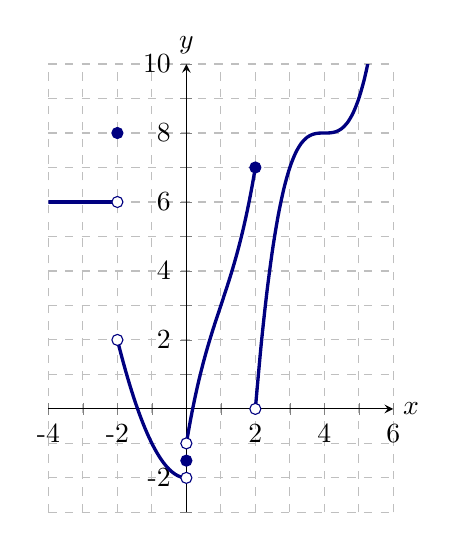
\begin{tikzpicture}
  \colorlet{penColor}{blue!50!black} % Color of a curve in a plot
\colorlet{gridColor}{gray!50} % Color of grid in a plot
\colorlet{background}{white} % Color of the page
	\begin{axis}[
           xmin=-4, xmax=6, ymin=-3, ymax=10,    
           unit vector ratio*=1 1 1,
           axis lines=middle, 
           xlabel=$x$, ylabel=$y$,
           y label style={at=(current axis.above origin),anchor=south},
           x label style={at=(current axis.right of origin),anchor=west},
           xtick={-4,...,6}, ytick={-3,...,10},
           xticklabels={-4,,-2,,0,,2,,4,,6}, yticklabels={,-2,,0,,2,,4,,6,,8,,10},
           grid=major,
           grid style={dashed, gridColor},
         ]
	  \addplot [very thick, penColor, smooth, domain=(-4:-2)] {6};
	  \addplot [very thick, penColor, smooth, domain=(-2:0)] {x^2-2};
         \addplot [very thick, penColor, smooth, domain=(0:2)] {(x-1)^3+3*(x-1)+3};
         \addplot [very thick, penColor, smooth, domain=(2:6)] {(x-4)^3+8};
         \addplot[color=penColor,fill=white,only marks,mark=*] coordinates{(-2,6)};  %% open hole
         \addplot[color=penColor,fill=background,only marks,mark=*] coordinates{(-2,2)};  %% open hole
         \addplot[color=penColor,fill=background,only marks,mark=*] coordinates{(0,-2)};  %% open hole
         \addplot[color=penColor,fill=background,only marks,mark=*] coordinates{(0,-1)};  %% open hole
         \addplot[color=penColor,fill=background,only marks,mark=*] coordinates{(2,0)};  %% open hole
         \addplot[color=penColor,fill=penColor,only marks,mark=*] coordinates{(-2,8)};  %% closed hole
         \addplot[color=penColor,fill=penColor,only marks,mark=*] coordinates{(0,-1.5)};  %% closed hole
         \addplot[color=penColor,fill=penColor,only marks,mark=*] coordinates{(2,7)};  %% closed hole
       \end{axis}
\end{tikzpicture}
\end{image}

\end{question}



\begin{question}
  What is the correct answer to this question?

  \begin{solution}
    \begin{multiple-choice}
      \choice[correct]{Correct answer}
      \choice{First Distractor}
      \choice{Second Distractor}
      \choice{Third Distractor}
    \end{multiple-choice}  
  \end{solution}
\end{question}

What other questions do you have about this lecture?
\begin{free-response}
\end{free-response}

\end{document}
